\chapter{Réseaux de neurones et traitement de données biomédicales non structurées}

\epigraph{\LARGE{``People should stop training radiologists now. It's just completely obvious that in five years deep learning is going to do better than radiologists.''}}{\LARGE{-- Geoffrey Hinton, 2016}}

La vision de Geoffrey Hinton, lauréat du prix Turing 2018 pour ses travaux en \gls{ia} et en \gls{dnn}, était peut-être un petit peu optimiste. Presque huit ans après cette prédiction, les radiologues n'ont pas été remplacés par l'\gls{ia} et continuent d'être formés. Cependant, il est important de remarquer que les méthodes \gls{ia} ont fait des progrès considérables et peuvent présenter des performances similaires aux radiologues, par exemple dans l'évaluation de radiographies de poumon (\cite{frauke_rudolf_ai_2023}). En juin 2023, il y a 238 produits médicaux basés sur IA pour la radiologie et autres méthodes d'imageries avec autorisation de mise sur le marché par la \gls{fda} (\cite{keith_j_dreyer_acr_2023}). Si l'\gls{ia} n'est pas encore prête à remplacer les radiologues et praticiens dans l'évaluation des données d'imagerie, elle est au moins maintenant capable de les assister afin de permettre un gain de temps et de précision dans l'évaluation des données.

Au cours de la dernière décennie, le domaine de l'\gls{ia} a été révolutionné par l'apparition des réseaux de neurones profonds (\textit{Deep Neural Networks}, DNN) grâce notamment aux travaux des Yann Lecun, Geoffrey Hinton et Yoshua Bengio. Cette nouvelle technologie d'\gls{ia} fait une promesse intéressante dans le cadre des données biomédicales: être capable de traiter automatiquement des données non structurées, c’est-à-dire sans devoir définir des descripteurs pertinents manuellement. Il est donc tout à fait pertinent d'explorer comment ces modèles peuvent être exploités pour le traitement des données biomédicales multimodales et hétérogènes. Dans ce chapitre, nous allons d'abord présenter le fonctionnement des réseaux de neurones. Puis nous allons étudier deux architectures spécifiques de réseaux de neurones qui ont permis la création de modèles d'analyse d'images (réseaux convolutifs) et de texte libres (réseaux de types \textit{transformers}).

\section{Réseaux de neurones profonds}
\subsection{Le concept de neurones et réseaux de neurones profonds}
Les réseaux de neurones sont un concept ancien qui a été décrit pour la première fois en 1958 par Frank Rosenblatt (\cite{rosenblatt_perceptron_1958}) sous sa plus simple forme nommée le perceptron, un réseau composé d'un seul neurone formel. Les réseaux de neurones reposent sur le concept bio-inspiré des neurones. La figure \ref{fig:neurons} présente les similarités entre un neurone biologique et un neurone formel en \gls{ia}. Le neurone biologique, par des processus biochimiques, capte les signaux d'entrée de l'environnement ou des neurones précédents par les dendrites. Ces signaux sont intégrés dans le corps cellulaire pour transmettre ou non un signal de sortie à travers l'axone vers d'autres neurones. Le neurone formel d'\gls{ia} est un modèle simplifié du neurone biologique qui mime leur fonctionnement. Ainsi le neurone formel intègre des entrées (x1, x2, x3 sur le schéma) comme les dendrites, il calcule un signal à transmettre (par la somme pondérée des entrées et la fonction d'activation) comme le corps cellulaire et transmet ce signal aux neurones suivants (sortie) comme les axones.

Le perceptron, réseau de neurones composé d'une seule couche d’un ou plusieurs neurones dans sa version plus avancée entre l'entrée et la sortie, n'est efficace que pour traiter des problèmes à séparation linéaire. Pour traiter des problèmes de classification plus complexes, il est nécessaire de multiplier les couches de neurones entre l'entrée et la sortie du réseau. Ces couches sont appelées couches "cachées", et forment ce qu'on appelle un réseau de neurones profond. La limite entre réseaux de neurones classiques (perceptron multi-couche) et réseaux de neurones profonds est floue. Certains auteurs peuvent considérer un réseau de neurones comme profond à partir de 3 couches cachées, pour d'autres, entre 10 couches et 100 sont nécessaires.

À l'instar du cerveau, les neurones formels (artificiels) sont présents en grand nombre dans les réseaux de neurones profonds et sont interconnectés selon une organisation précise, cette organisation se nomme l'architecture du réseau.

\begin{figure}[htbp]
 \centering
 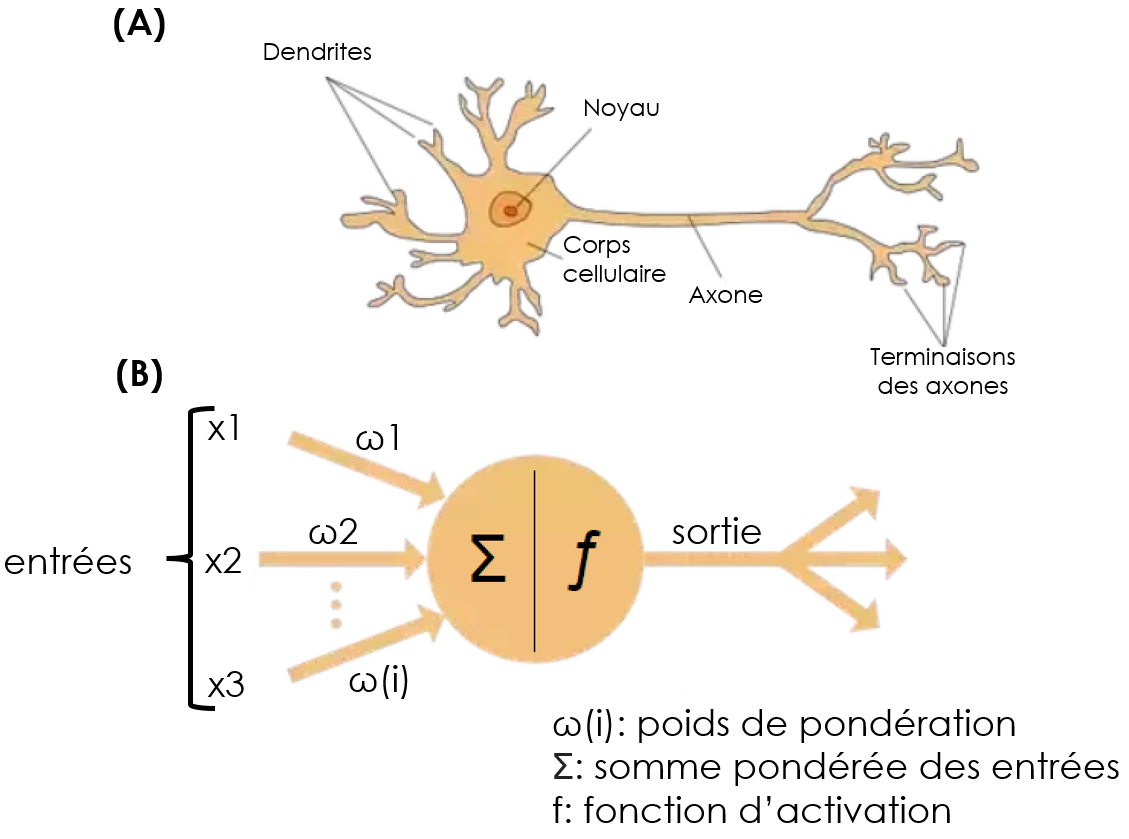
\includegraphics[width=0.7\textwidth]{figures/neuronne.png}
 \caption[Comparaison du neurone biologique et du neurone formel]{\textbf{Comparaison du neurone biologique et neurone formel. (A)} Représentation schématique du neurone biologique. \textbf{(B)} Représentation schématique du neurone formel utilisé en \gls{ia}}
 \label{fig:neurons}
\end{figure}

\subsection{Les réseaux de neurones: une diversité d'architectures}
La multiplication du nombre des neurones dans un réseau de neurones et de leur interconnexion permet de constituer des architectures spécifiques qui confèrent des compétences particulières au réseau de neurones comme l'intégration d'informations locales (pour l'imagerie par exemple grâce à la convolution, \cite{fukushima_neocognitron_1980}), l'intégration d'informations globales (pour l'analyse de séquences comme des phrases par exemple grâce aux \textit{transformers}, \cite{vaswani_attention_2017}), des mécanismes de "mémoires" (pour l'analyse de textes par exemple grâce à la \textit{Long short-term memory}, LSTM, \cite{hochreiter_long_1997}) ou encore des capacités génératives (pour la génération d'images par exemple grâce aux réseaux antagonistes génératifs (GAN) et aux modèles de diffusion). La figure \ref{fig:dnn_archi} (\cite{leijnen_neural_2016}) présente graphiquement quelques architectures de réseaux de neurones communes. On y retrouve le perceptron (P), le perceptron multi-couche (DFF), le réseau LSTM, le \gls{dnn} convolutif (DCN) et les réseaux GAN.

\begin{figure}[htbp]
 \centering
 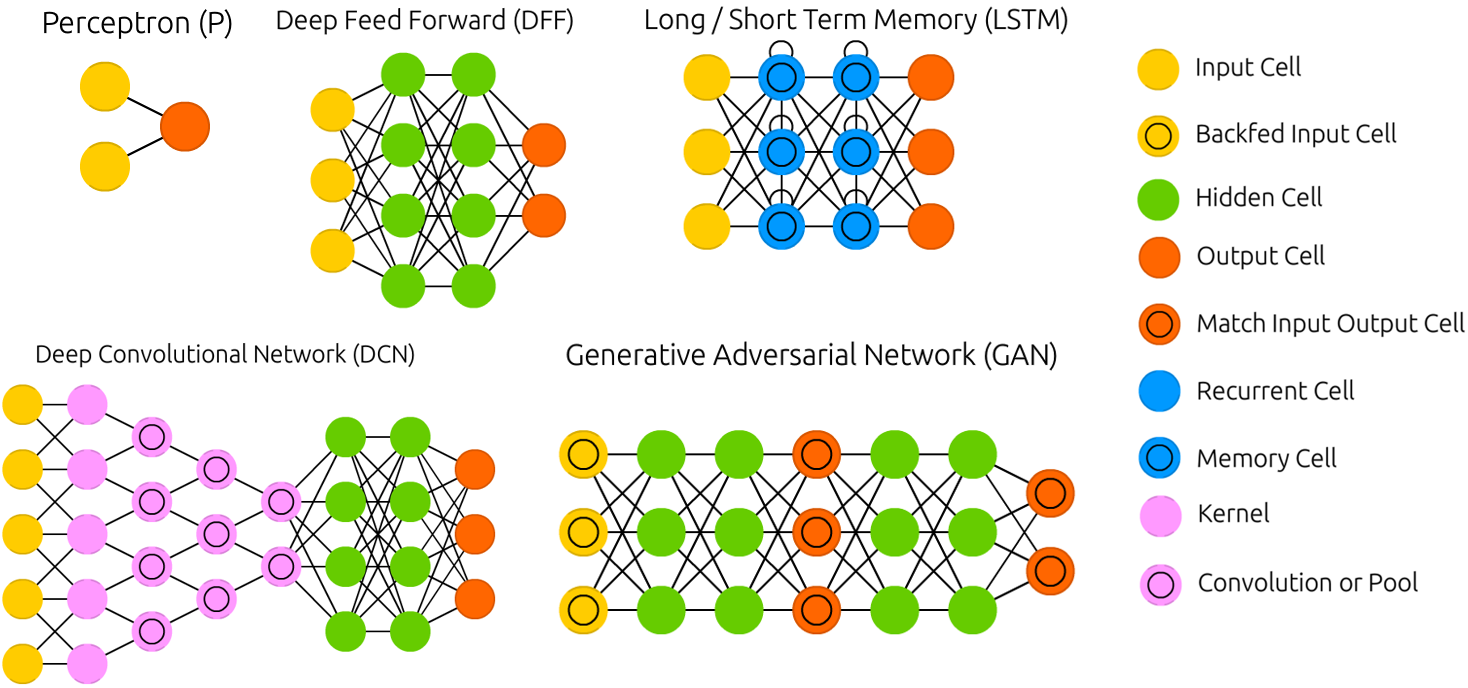
\includegraphics[width=0.9\textwidth]{figures/dnn_archi.png}
 \caption[Représentation de différentes architectures de \gls{dnn}]{\textbf{Représentation de différentes architectures de \gls{dnn}}. Le type de neurones, leurs organisations en couches et les interconnections qui les lient définissent des architectures qui leur confère certaines capacités comme le traitement d'images (DCN) où encore la mémoire à court terme (LSTM). (modifié de \cite{leijnen_neural_2016})}
 \label{fig:dnn_archi}
\end{figure}


\subsection{L'entrainement d'un réseau de neurones}
L'entrainement d'un réseau de neurones consiste à trouver, pour chaque neurone qui le compose, la valeur de poids ($\omega$) pour chaque entrée optimale pour remplir la tâche qui lui est assignée. Pour cela un réseau de neurones a besoin de deux éléments: (i) une fonction de cout permettant d'évaluer son niveau d'erreur de classification et (ii) une méthode qui permet de modifier les poids des connexions neuronales pour réduire cette erreur grâce à la descente de gradient et à la rétropropagation.

\subsubsection{Fonction de cout}
La fonction de cout permet de fournir une mesure quantitative des performances d'un réseau de neurones profonds. Elle mesure la divergence entre les prédictions réalisées par le modèle et les labels véritables des données. Cette fonction varie en fonction de la tâche à réaliser, pour une tâche de régression, un choix courant est l'utilisation de l'erreur quadratique moyenne (\textit{mean square error}, MSE). Pour une classification, il est commun d'utiliser l'entropie croisée binaire (\textit{binary cross entropy}). 

Dans tous les cas, plus cette valeur est élevée, plus les prédictions du modèle divergent de la vérité de terrain, plus cette valeur est proche de 0, plus les prédictions du modèle sont exactes. Ainsi, l'objectif de l'entrainement d'un réseau de neurones est de faire converger la valeur de la fonction de cout du jeu d'entrainement et du jeu de validation vers 0. 

La figure \ref{fig:loss_func} présente un exemple théorique de valeurs de fonction de cout au cours de l'entrainement d'un modèle \gls{dnn}. Dans cet exemple, l'écart tout au long de l'apprentissage entre le jeu de validation et d'entrainement est important à des fins de visualisation, en pratique, les deux courbes doivent presque se superposer. On observe ici qu'au cours de l'entrainement cette valeur converge vers 0. Cependant, au bout d'un moment, la valeur pour le jeu d'évaluation remonte tandis que celle du jeu d'entrainement continue de baisser, il s'agit du phénomène de sur-apprentissage, le modèle cesse d'apprendre à généraliser et apprend simplement par cœur le jeu d'entrainement. Dès lors, il est nécessaire d'arrêter l'apprentissage au moment où la valeur du jeu de validation augmente, il s'agit de ce qu'on appelle l'arrêt prématuré pour éviter le sur-apprentissage.

\begin{figure}[htbp]
 \centering
 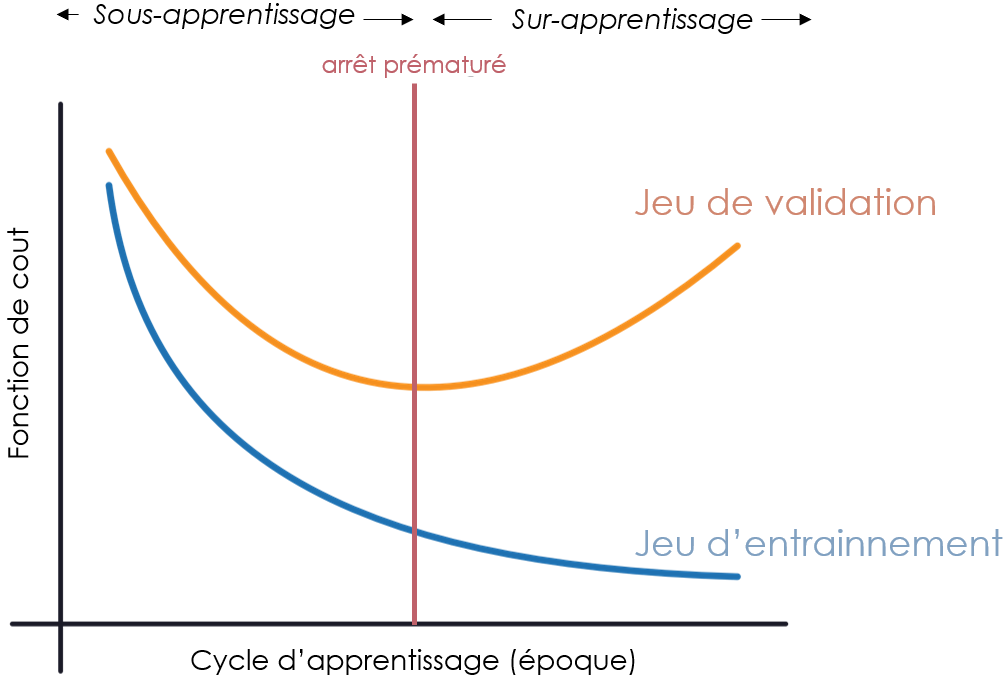
\includegraphics[width=0.7\textwidth]{figures/loss_function.png}
 \caption[Schéma d'un exemple de fonction de coût lors d'un entraînement]{\textbf{Schéma d'un exemple de fonction de coût lors de l'entrainement d'un \gls{dnn}.} Au cours de l'entrainement, la fonction de cout baisse après chaque cycle d'apprentissage à la fois pour le jeu d'entrainement et le jeu de validation. Puis celle du jeu d'entrainement continu de baisser tandis que celle du jeu de validation augmente: le modèle commence un sur-apprentissage, il est nécessaire de stopper l'entrainement.}
 \label{fig:loss_func}
\end{figure}

\subsubsection{Rétropropagation et descente de gradient}
La figure \ref{fig:retropop} (\cite{scalzitti_nouvelle_2021}) présente le mécanisme de rétropropagation. Lors d'une prédiction, les signaux sont propagés vers l'avant (nommé \textit{forward pass}) à partir de la couche d'entrée jusqu'à la couche de sortie, puis l'erreur est ensuite calculée grâce à la fonction de cout. Lors de l'entrainement, le chemin inverse est réalisé en propageant le gradient de l'erreur pour identifier les neurones responsables des erreurs (\textit{backward pass}) (\cite{lecun_deep_2015}). Ce processus de rétropropagation permet d'identifier les neurones responsables des erreurs dont les paramètres doivent être modifiés pour réduire la fonction de cout.

\begin{figure}[htbp]
 \centering
 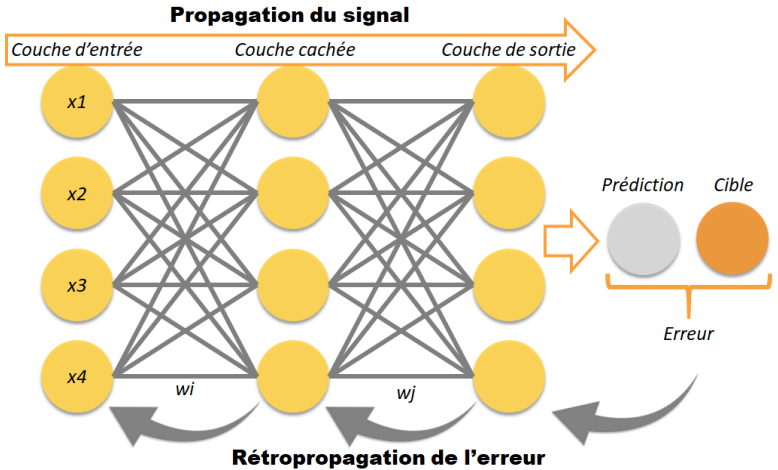
\includegraphics[width=0.7\textwidth]{figures/retro_propagation.png}
 \caption[Schéma de la rétro-propagation]{\textbf{Schéma de la propagation du signal lors de la prédiction et de la rétropropagation lors de l'entrainement}. Lors d'une prédiction, le signal est propagé vers l'avant à travers les neurones, puis une erreur est calculée. Cette erreur est ensuite propagée dans le sens inverse à travers les neurones, c'est la rétropropagation. (\cite{scalzitti_nouvelle_2021})}
 \label{fig:retropop}
\end{figure}

Après avoir identifié les neurones à modifier (et donc avoir calculé le gradient de chaque neurone), leurs poids vont être ajustés grâce à la méthode de la descente de gradient. La figure \ref{fig:grad_descent} présente le fonctionnement de la descente de gradient. À chaque étape d'apprentissage, les poids des neurones (ici un seul poids pour un neurone sur la figure) sont mis à jour dans la direction négative du gradient, ce qui a pour effet de réduire la valeur de la fonction de cout. Cette modification des poids est proportionnelle à un paramètre nommé le pas d'apprentissage (\textit{learning rate}). Ces cycles d'apprentissage vont se répéter jusqu'à atteindre un minimum (global ou local) dans la fonction de cout, indiquant un poids optimal pour la fonction de cout (et donc la tâche à réaliser).

\begin{figure}[htbp]
 \centering
 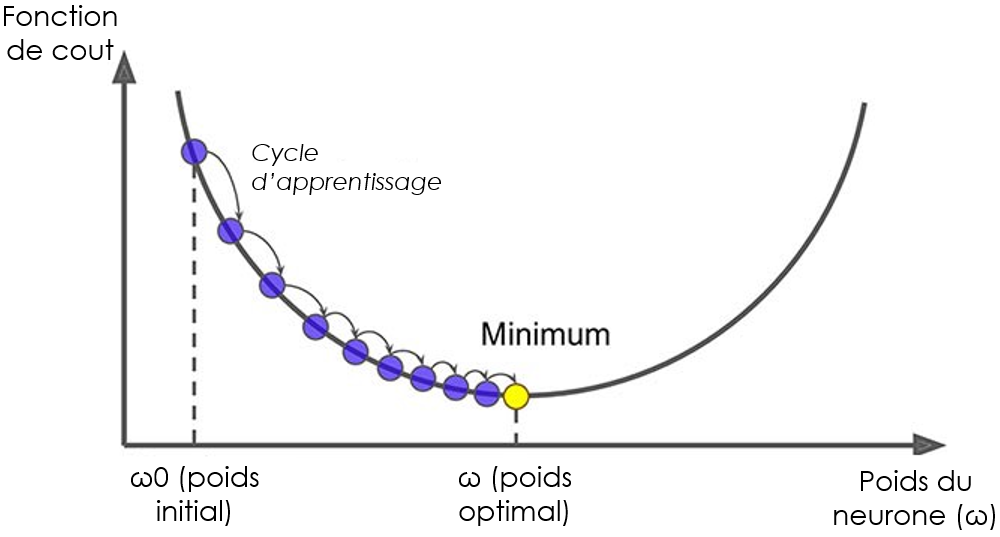
\includegraphics[width=0.7\textwidth]{figures/gradient_descent.png}
 \caption[Schéma de la descente de gradient pour un poids d'un neurone]{\textbf{Schéma de la descente de gradient pour un poids d'un neurone}. À chaque cycle d'apprentissage, le poids du neurone est mis à jour jusqu'à un minimum local qui minimise la fonction de cout.}
 \label{fig:grad_descent}
\end{figure}

La rétropropagation et la descente de gradient permettent l'apprentissage de réseaux de neurones composés de centaines de milliers, voire de millions et même de milliards de neurones. La taille des \gls{dnn} est très variable en fonction des architectures et de la tâche à effectuer. Ainsi, les couts en matière de calcul pour leur entrainement (le calcul des gradients et la mise à jour des poids) peuvent devenir très importants. Dans la prochaine sous-section, nous allons présenter des exemples de réseaux et d'architectures de \gls{dnn} et les ressources informatiques associées nécessaires à leur utilisation.

\subsection{Nombre de paramètres et ressources informatiques}
Il existe un lien de proportionnalité entre la taille (en nombre de neurones) d'un \gls{dnn}, sa précision et les ressources de calcul nécessaires à son entrainement et aux prédictions. En théorie, plus un réseau est grand, plus importante est sa capacité à capturer des relations complexes entre les données et meilleure est sa précision. Le tableau \ref{table:dnn-size} (\cite{chollet_keras_2023}) présente plusieurs architectures utilisées pour la classification d'images. On observe que pour une même architecture, augmenter le nombre de paramètres permet d'obtenir de meilleures performances, mais au détriment d'un temps d'inférence plus long. Cependant, lors d'une comparaison de deux architectures différentes, la relation performance - nombre de paramètres n'est pas forcément vérifiée. Les réseaux EfficientNet (architecture de classification d'image développée en 2020 pour améliorer les ResNet \cite{tan_efficientnet_2020}) performent mieux que les réseaux ResNet (architecture de 2015 \cite{he_deep_2015}) avec un nombre de paramètres moindre, cependant une règle qui reste vérifiée dans toutes les conditions: les réseaux qui performent le mieux ont un temps d'inférence plus long, quelle que soit leur architecture.

\begin{table}[htbp]
\centering
\begin{tabular}{|l|c|c|c|} 
 \hline
 Architecture & Paramètres (millions) & Précision (ImageNet, \%) & Temps d'inférence (ms) \\
 \hline
MobileNetV2 & 3,5 & 71,3 & 3,8 \\
\hline
ResNet50V2 & 25,6 & 74,9 & 4,6 \\ 
ResNet101V2 & 44,7 & 77,2 & 5,4 \\ 
ResNet152V2 & 60,4 & 78,0 & 6,6 \\
\hline
EfficientNetB1 & 7,9 & 79,1 & 5,6 \\
EfficientNetB2 & 9,2 & 80,1& 6,5 \\
EfficientNetB3 & 12,3 & 81,6 & 8,8 \\
 \hline
\end{tabular}
\caption[Tableau de comparaison d'architectures de \gls{dnn} et performances]{\textbf{Tableau de comparaison d'architectures de \gls{dnn} et performances}. Pour un même type d'architecture, l'augmentation du nombre de paramètres améliore les performances, mais réduit aussi la vitesse d'inférence. Cependant un nombre de paramètres plus élevé ne signifie pas forcément de meilleures performances quand on compare deux architectures différentes. (\cite{chollet_keras_2023})} 
\label{table:dnn-size}
\end{table}

L'entrainement et l'inférence des \gls{dnn} se réalise sur un matériel informatique spécialisé nommé \gls{gpu}. Au contraire des processeurs centraux (CPU) qui sont conçus pour des opérations séquentielles, les \gls{gpu} permettent de réaliser un grand nombre d'opérations mathématiques en parallèle. Or, les opérations principales nécessaires pour l'entrainement et l'inférence d'un \gls{dnn} sont des calculs matriciels et donc intrinsèquement parallélisables. La caractéristique limitante des \gls{gpu} concerne leur mémoire disponible (VRAM). En effet, plus le modèle de \gls{dnn} est grand, plus il possède de paramètres, plus il va être demandeur en mémoire, car il est nécessaire de pouvoir garder l'ensemble des poids à optimiser en mémoire. 

Ainsi, s'il est possible d'entrainer et de faire de l'inférence de modèles de taille raisonnable sur des \gls{gpu} accessibles au grand public, cette tâche devient complexe, voire impossible, pour des modèles de très grande taille, sans engager des couts de plusieurs centaines de milliers d'euros de matériel. À titre d'exemple, il est possible d'héberger et d'entrainer des modèles de quelques dizaines de millions de paramètres à quelques milliards de paramètres (tel que Resnet50 (25~millions de paramètres) et LLaMA-7B (7~milliards de paramètres) sur un seul \gls{gpu} grand public (16 à 24 Go de mémoire). 

Parmi les modèles les plus grands à ce jour, on retrouve les modèles développés pour l'analyse de langages (\gls{llms}) présentés dans une prochaine section (\ref{chap2_llms}). Ces modèles atteignent une taille de plusieurs dizaines voire des centaines de milliards de paramètres: par exemple GPT-3 d'OpenAI (175~milliards de paramètres) (\cite{brown_language_2020}) ou LLaMA de META (65~milliards de paramètres) (\cite{touvron_llama_2023}). Ce type de modèles demande l'utilisation de plusieurs \gls{gpu} haut de gamme (4 à 8) pour leur hébergement et inférence. À titre indicatif, un cluster composé de 4 \gls{gpu} H100 (40,000€ pièce), coute 17.9\$/heure d'utilisation, soit environ 13 000\$ d'hébergement mensuel pour un modèle accessible en continu. Un travail d'optimisation pour réduire la taille des modèles tout en conservant leurs performances est donc nécessaire pour permettre d'utiliser ce type d'architecture et de dépasser les challenges liés à leur hébergement.

\section{L'analyse d'imagerie et de séquences par réseau neuronal convolutif}
L'architecture des réseaux de neurones convolutifs (CNN) permet l'analyse et l'exploitation de données de type image brute. Cette architecture est majoritairement utilisée pour la classification et segmentation d'images, mais elle est aussi capable d'exploiter des données de types séquences (phrases, séquences génomiques...). Elle est basée sur les travaux réalisés sur le cortex visuel de chats et de primates dans lesquels il a été démontré que chaque neurone du cortex visuel captait une information locale, dans un champ visuel réduit. De plus, chaque neurone n'est en mesure de capter qu'une orientation de ligne (horizontale, verticale ou oblique) (\cite{hubel_receptive_1959, hubel_single_1959}). À partir de ces travaux, le concept de couches convolutives pour les réseaux de neurones a été formulé (\cite{fukushima_neocognitron_1980}) et a permis la construction du premier \gls{dnn} convolutif pour reconnaitre des numéros sur des chèques de banque grâce au réseau LeNet-5 (\cite{lecun_gradient-based_1998}). Vingt-cinq ans plus tard, en 2023, les \gls{cnn} sont encore utilisés pour l'analyse de données d'imagerie biomédicale (\cite{holscher_next-generation_2023, ker_automated_2019}).
 
\subsection{Fonctionnement des couches convolutives pour l'analyse d'images}
Pour simuler le comportement des neurones du cortex visuel, les neurones d'une couche convolutive ne sont connectés qu'à une zone restreinte d'une image, généralement sous forme d'un carré de pixels. La figure \ref{fig:conv_simple} (\cite{aurelien_geron_hands-machine_2019}) présente schématiquement la liaison de trois neurones répartis sur deux couches convolutives par rapport à une image de base. On observe que ces neurones n'ont accès qu'à une portion de l'image, donc à une information locale. 

\begin{figure}[htbp]
 \centering
 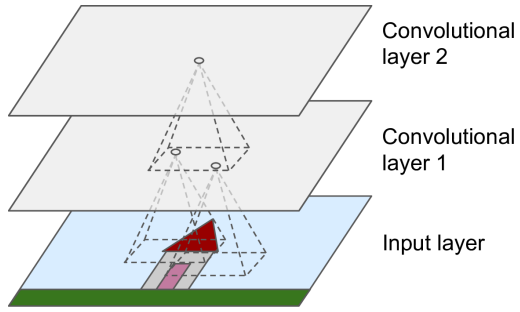
\includegraphics[width=0.7\textwidth]{figures/conv_simple.png}
 \caption[Schéma de la connection des neurones convolutifs à une image]{\textbf{Schéma de la connexion des neurones convolutifs à une image.} Les neurones ne sont connectés qu'à une portion locale de l'image sous la forme d'un carré de pixels. (modifiée de \cite{aurelien_geron_hands-machine_2019})}
 \label{fig:conv_simple}
\end{figure}

La convolution consiste à appliquer un filtre à une entrée pour produire une carte de caractéristiques (\textit{feature map}). Ainsi les neurones de la couche convolutive ont en entrée une portion de l'image et vont appliquer un filtre pour extraire une information de cette portion (une ligne horizontale, une texture, un contraste...). Le but de l'entrainement du \gls{cnn} est, pour chaque neurone, de trouver les filtres optimaux à utiliser pour extraire l'information pertinente à la classification de l'image. Autrement dit, chaque neurone va apprendre à extraire une information pertinente de la zone à laquelle il a accès.

La figure \ref{fig:conv_simple} (\cite{aurelien_geron_hands-machine_2019}) est simpliste, car elle représente les couches convolutives comme composées d'une seule couche de neurones et donc un seul filtre. En réalité, comme présentée en figure \ref{fig:conv_complex} (\cite{aurelien_geron_hands-machine_2019}), chaque couche convolutive est composée de plusieurs filtres (couches de neurones formant des cartes de caractéristique). Chacune de ces cartes de caractéristique (\textit{feature map}) est reliée aux précédentes afin d'extraire des caractéristiques très diverses (des formes horizontales, verticales, de la texture, du contraste...).

\begin{figure}[htbp]
 \centering
 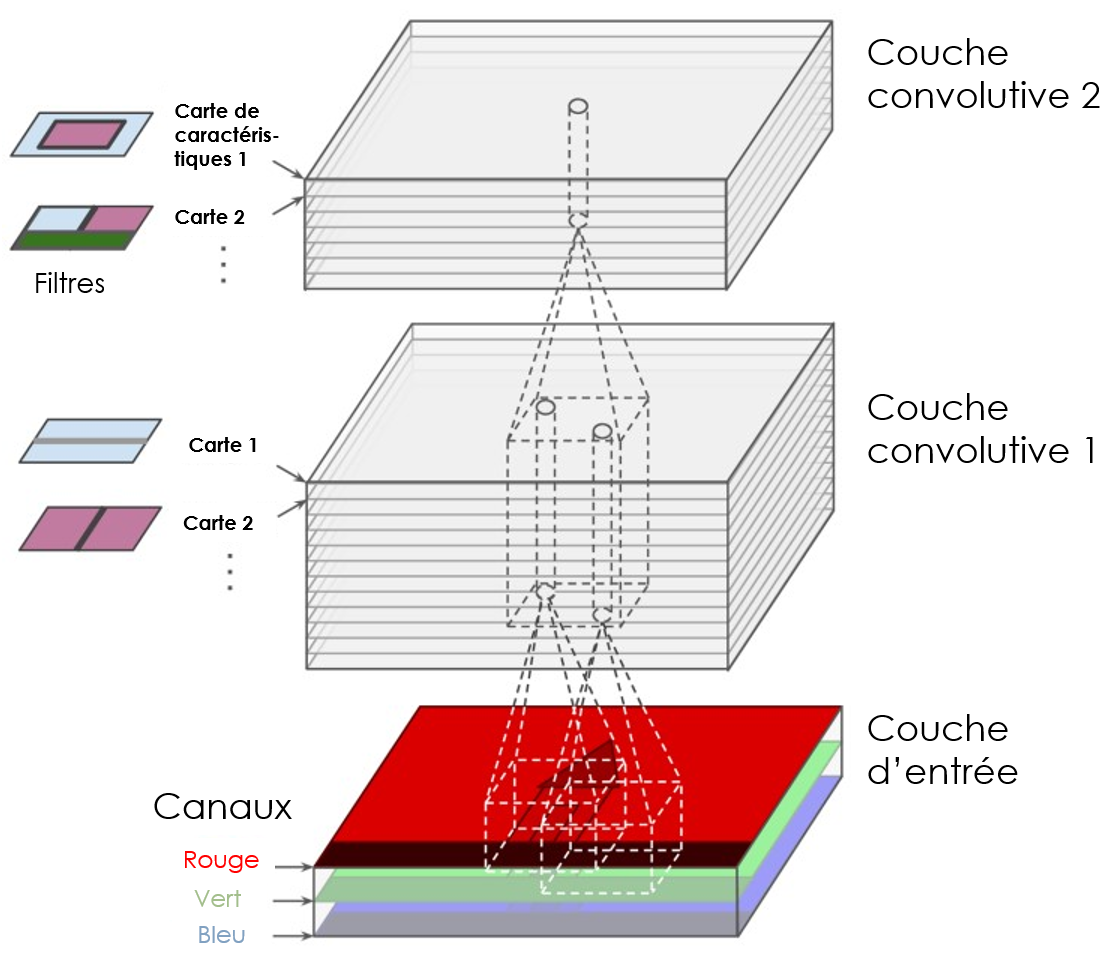
\includegraphics[width=0.7\textwidth]{figures/conv_complex.png}
 \caption[Schéma des couches convolutives]{\textbf{Schéma des couches convolutives complexes}. Chaque couche convolutive est en réalité composée de plusieurs filtres, chacun générant une carte de caractéristique propre. (modifiée de \cite{aurelien_geron_hands-machine_2019})}
 \label{fig:conv_complex}
\end{figure}

Enfin pour simplifier les couts de calcul et réduire la mémoire nécessaire, après un bloc de convolution, une étape de \textit{max-pooling }(en français: sous-échantillonnage maximal) est réalisée. Cette technique permet de réduire la dimensionnalité des cartes de caractéristiques en préservant les informations essentielles. La figure \ref{fig:max-pool} (\cite{aurelien_geron_hands-machine_2019}) présente le fonctionnement de cette méthode. La carte de caractéristique est divisée en carré non chevauchant et la valeur maximale de chaque carré est sélectionnée. Par exemple, si on a une carte de caractéristique de taille 4x4 et qu'on réalise un \textit{max pooling} de taille 2, on obtient une carte de caractéristique de taille 2x2, c'est-à-dire quatre fois plus petite.

\begin{figure}[htbp]
 \centering
 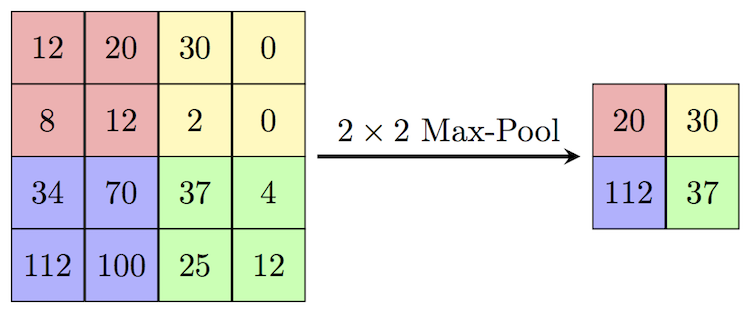
\includegraphics[width=0.5\textwidth]{figures/max-pool.png}
 \caption[Technique de max-pooling]{\textbf{Schéma de la technique de \textit{max-pooling} pour réduire la dimensionnalité d'une matrice}. Le max-pooling permet de réduire la dimension d'une carte de caractéristique en conservant les informations importantes, réduisant ainsi les couts de calcul. (\cite{aurelien_geron_hands-machine_2019})}
 \label{fig:max-pool}
\end{figure}

Pour finir, la figure \ref{fig:cnn_archi} (\cite{aurelien_geron_hands-machine_2019}) présente la structure typique d'un \gls{cnn}. Un \gls{cnn} consiste en l'enchainement de couches de convolution et de \textit{max-pooling} avant les couches de classification (\textit{fully connected}, une couche de neurones où tous les neurones sont connectés à la couche précédente.). Le but de cette architecture est de réduire la dimensionnalité de l'image tout en augmentant la profondeur (c'est-à-dire le nombre d'informations extraites par position). Par exemple, pour une image de 512x512 (c'est-à-dire 262 144 pixels), si en sortie de couches convolutives on obtient une matrice de taille (4x4x128, soit 2048 points), cela signifie que nous avons extrait 128 caractéristiques pour chacune des 16 zones de l'image. Ces 128 caractéristiques par zone vont être utilisées pour classer l'image.

\begin{figure}[htbp]
 \centering
 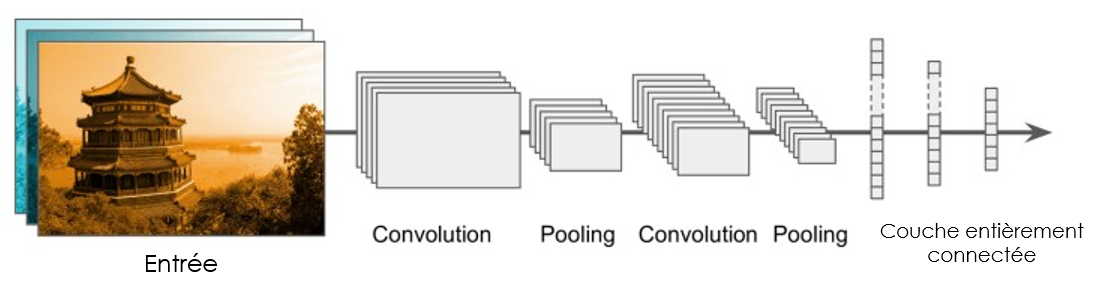
\includegraphics[width=0.7\textwidth]{figures/cnn_simple.png}
 \caption[Schéma de la structure d'un \gls{cnn} typique]{\textbf{Schéma de la structure d'un \gls{cnn} typique. } Une architecture de \gls{cnn} typique consiste en un enchaine de couche convolutives et de max-pooling (extraction d'information), puis d'une couche finale entièrement connectée pour la classification (modifiée de \cite{aurelien_geron_hands-machine_2019})}
 \label{fig:cnn_archi}
\end{figure}

\subsection{Modèle généraliste pour l'histologie}
La couche de neurones convolutifs représente la brique de base des \gls{cnn}. À partir de cette architecture de réseau, il est possible de réaliser diverses tâches en variant légèrement l'organisation des couches. Dans cette section, nous présentons deux exemples d'utilisation des \gls{cnn} pour le traitement de données biomédicales.

\subsubsection{Segmentation d'images histologiques: détection de cellules avec Cellpose}
La segmentation d'une image consiste à diviser l'image en groupes de pixels (segment) dans l'objectif d'obtenir les coordonnées d'éléments d'intérêts. Par exemple, dans le cadre d'une image de coupe histologique (image de tissus au microscope), il peut être intéressant de mesurer le nombre de cellules présentes et leur taille. Pour automatiser ce processus, il est nécessaire d'avoir recours à un réseau de neurones capable de réaliser de la segmentation d'image.

Cellpose (\cite{stringer_cellpose_2021}), développé par Carsen Stringer en 2021, est un modèle de segmentation généraliste, conçu pour être capable de segmenter les cellules de n'importe quelle coupe histologique. La figure \ref{fig:cellpose_archi} présente l'architecture du modèle ainsi qu'un exemple d'image histologique et de résultat de segmentation. L'architecture de \gls{cnn} utilisée se nomme U-Net (\cite{ronneberger_u-net_2015}) structurée comme un U avec un chemin de contraction (encodeur, grâce à la convolution) et un chemin d'expansion (décodeur grâce à la "\textit{upconvolution}"). Cette architecture permet à partir de l'image d'entrée, composée de cellules en microscopie à fluorescence, de générer un masque de segmentation, de la même taille que l'image d'entrée. Ce masque de segmentation est une abstraction de l'image d'entrée où les pixels de chaque objet (cellules) sont marqués avec un identifiant unique. Ainsi il est possible à partir de ce masque de compter ou de mesurer la taille des cellules.

\begin{figure}[htbp]
 \centering
 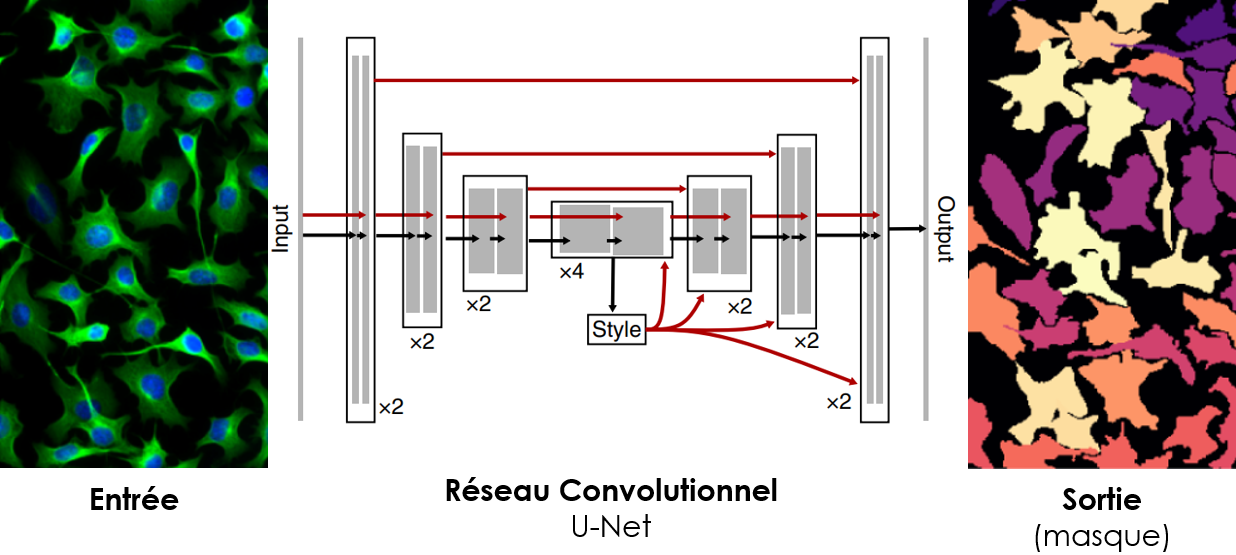
\includegraphics[width=0.8\textwidth]{figures/cellpose_archi.png}
 \caption[Architecture du réseau convolutionel de CellPose]{\textbf{Architecture du réseau convolutif de CellPose}. Cellpose est composé d'un réseau CNN de type U-Net. Cette architecture en forme de U est composée d'un chemin de contraction (un encodeur grâce à la convolution qui extrait des informations de l'image) puis d'un chemin d'expansion (décodeur grâce à l'\textit{upconvolution}) qui reconstitue une image simplifiée, sous la forme d'un masque de segmentation. (modifié de \cite{stringer_cellpose_2021})}
 \label{fig:cellpose_archi}
\end{figure}

\subsubsection{Analyse de séquences: prédiction de sites d'épissage avec Spliceator}
En plus du traitement d'images, les \gls{cnn} peuvent être utilisés pour traiter des données de type séquences nucléotidiques. Au sein de notre équipe, en 2021, l'outil Spliceator a été développé (\cite{scalzitti_spliceator_2021}) pour analyser des séquences génomiques et prédire les sites d'épissages. La figure \ref{fig:splice_archi} présente la structure du \gls{cnn} entrainé pour cette tâche de classification. Le \gls{cnn} entrainé est capable de prédire les sites d'épissage de plus de 100 espèces vivantes avec une précision de plus de 90\%. L'architecture utilisée par Spliceator est une architecture classique de \gls{cnn} avec trois blocs convolutifs puis une couche \textit{fully-connected} pour la classification, identique à l'exemple en figure \ref{fig:cnn_archi}. Cette architecture a permis d'entrainer un modèle capable de prendre en compte un contexte jusqu'à 600 nucléotides en amont et en aval du site d'épissage à évaluer.

\begin{figure}[htbp]
 \centering
 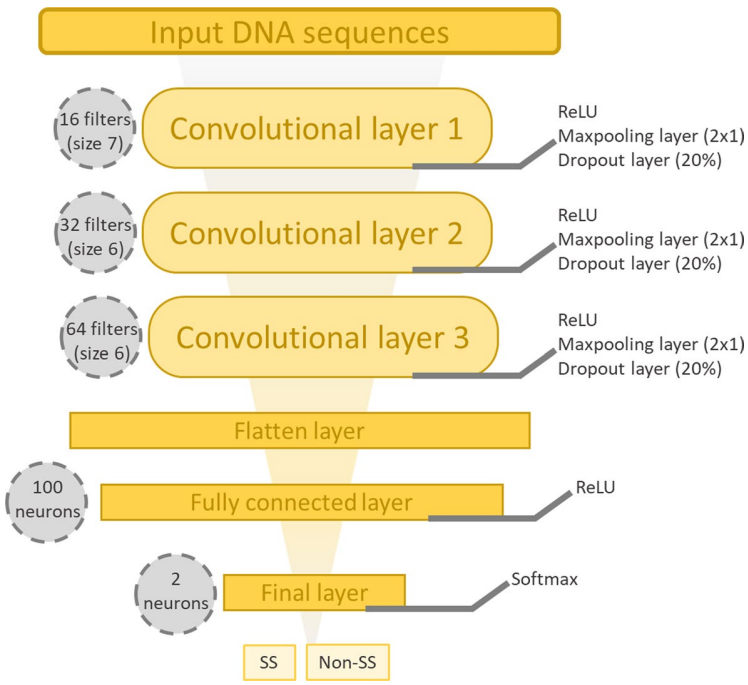
\includegraphics[width=0.66\textwidth]{figures/spliceator_nn.png}
 \caption[Architecture du réseau convolutionel de Spliceator]{\textbf{Architecture du réseau convolutif de Spliceator}. Une suite de trois couches convolutives sont utilisées pour extraire les caractéristiques qui constituent les sites d'épissages puis une couche entièrement connectée utilise ces caractéristiques pour apprendre à reconnaitre les sites d'épissages. (\cite{scalzitti_spliceator_2021})}
 \label{fig:splice_archi}
\end{figure}

Bien que les \gls{cnn} soient capables d'intégrer de l'information locale pour mimer le fonctionnement du contexte visuel pour une analyse d'image, la détection et l'intégration d'interactions longue distance demeurent un problème majeur. Cette limite pose problème dans le cadre de l'analyse de séquences. Par exemple, si l’on cherche à prédire l'expression d'un gène, il existe des signaux à longue distance qui modulent cette expression, tels que les séquences \textit{enhancers}, dont plus de la moitié sont situées à des distances de 50 000 paires de bases ou plus du gène modulé (\cite{chepelev_characterization_2012}). De même pour l'analyse de texte, une information importante pour la compréhension d'une phrase peut être située bien en amont à plusieurs dizaines, voir des centaines de mots.

Ainsi pour construire des architectures de \gls{dnn} capables de s'attaquer aux défis de l'analyse de textes et de séquences, il est nécessaire d'avoir des modules capables de prendre en compte le contexte global. Ceci est rendu possible grâce à l'architecture nommée \textit{transformer} (\cite{vaswani_attention_2017}), qui est présentée dans la prochaine section.

\section{Architecture transformer et la révolution des modèles linguistiques de grande taille}
Les \textit{transformers} sont des architectures qui ont révolutionné le domaine de l'analyse de séquence et de texte depuis leur première description (\cite{vaswani_attention_2017}). Cette architecture a permis de dépasser toutes les limitations des architectures précédentes, en particulier les limites concernant leur faible mémoire à longue distance. Les modèles \textit{transformers} sont des modèles dits de séquence à séquence (\textit{Seq2Seq}), qui prennent en entrée une séquence (une phrase) et produisent en sortie une autre séquence (par exemple la phrase traduite). Pour comprendre comment les \textit{transformers} fonctionnent et quelles sont leurs implications, deux notions sont nécessaires: la structure encodeur-décodeur et les mécanismes d'attention.

\subsection{La structure encodeur-décodeur et l'attention multitête}
La structure encodeur-décodeur est au cœur de nombreuses architectures et est vitale pour une multitude de tâches telles que la génération de texte ou la traduction. L'idée derrière cette structure est de compresser l'information d'entrée en un vecteur numérique de taille définie, nommé "état caché" (figure \ref{fig:encoder_decoder}). Puis le décodeur, à partir de cet état caché, va générer une séquence (par exemple une phrase) qui correspond à cet état caché. Lors de l'entrainement d'un réseau encodeur-décodeur, les paramètres de l'encodeur et du décodeur sont ajustés pour minimiser la fonction de cout. 

Par exemple, imaginons que l'on veuille construire un réseau de traduction du français vers l’anglais (figure \ref{fig:encoder_decoder}). Pour cela, on va utiliser comme données d'entrainement des couples de phrases françaises (entrée) et anglaises (cible). L'entrainement consiste à apprendre à l'encodeur à représenter numériquement les phrases françaises en extrayant les informations les plus pertinentes. L'entrainement du décodeur consiste à apprendre comment à partir de cet état caché, reconstruire la phrase anglaise attendue.

Cependant, cette structure possède des limites. En effet, pour des phrases très longues ou des paragraphes, l'encodeur n'est pas nécessairement en mesure de représenter toutes les informations pertinentes dans l'état caché qui possède une taille fixe, ainsi de l'information pourrait être perdue. Les mécanismes d'attention à l'œuvre dans les \textit{transformers} permettent de pallier cette limite.

\begin{figure}[htbp]
 \centering
 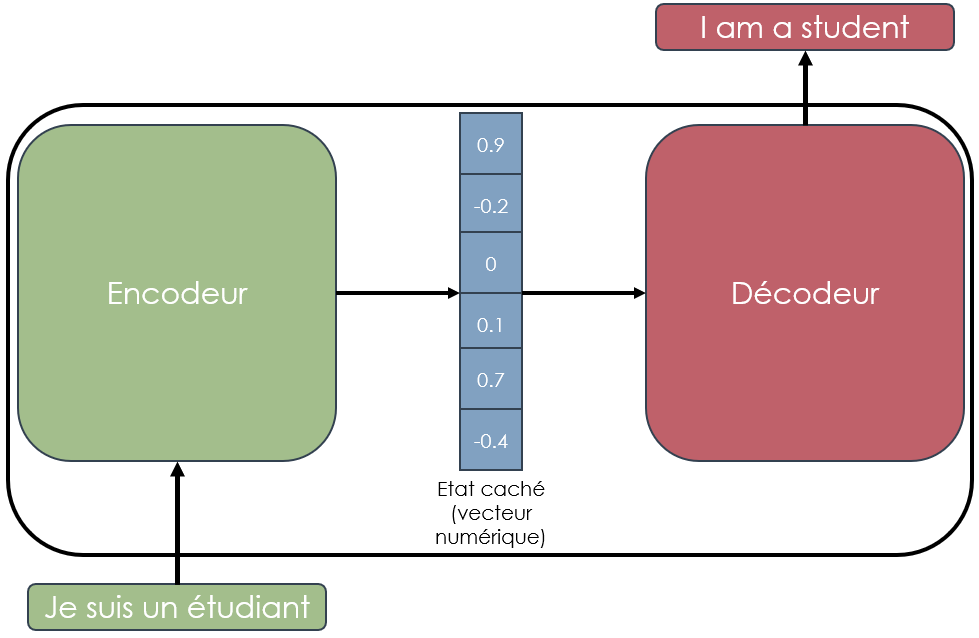
\includegraphics[width=0.66\textwidth]{figures/encoder_decoder.png}
 \caption[Schéma de la structure encodeur-décodeur]{\textbf{Schéma de la structure encodeur-décodeur}. Cette structure permet l'encodage d'une donnée dans un état caché puis son décodage pour la traduction par exemple. }
 \label{fig:encoder_decoder}
\end{figure}

Dans un \textit{transformer}, les encodeurs et les décodeurs sont multiples (au total de 6 dans le papier les décrivant pour la première fois) et ils sont composés de mécanismes d'auto-attention (figure \ref{fig:encoder_attention}). Le mécanisme d'auto-attention permet à n'importe quel élément de la séquence (mot de la phrase) d'être influencé par les autres éléments. C'est-à-dire que le premier mot d'une phrase peut avoir une influence sur le dernier, ce qui permet une influence longue distance. Mathématiquement, cela est possible par la création pour chaque mot de la phrase de trois vecteurs: requête (Q), clé (K) et valeur (V) (non représenté sur la figure \ref{fig:encoder_attention}). Puis par un produit scalaire, un score d'attention est calculé pour tous les couples de mots présents dans la phrase (c'est donc un processus quadratique).

Ces mécanismes d'attention sont divisés en plusieurs têtes, qui permettent lors de l'entrainement de spécialiser chacune des têtes d'attention sur un aspect spécifique de l'entrée. Par exemple, dans le cadre d'un texte, une tête peut être spécialisée dans la syntaxe et une autre dans des aspects sémantiques. 
La multiplicité des \textit{transformers} et les mécanismes d'attention multitête permettent aux réseaux de traiter des données de grandes tailles sans perte d'informations, c'est-à-dire avec une grande "mémoire". Ainsi, cela permet de détecter et d'intégrer lors des prédictions réalisées des informations à longue distance, là où la convolution ne permettait d'intégrer que des informations locales.

\begin{figure}[htbp]
 \centering
 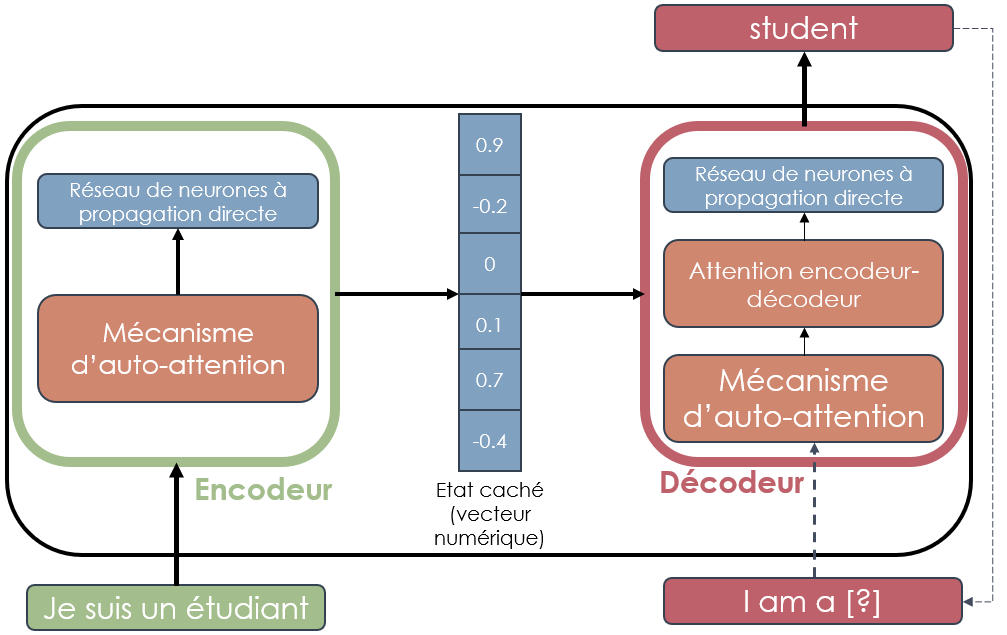
\includegraphics[width=0.66\textwidth]{figures/encoder_attention.png}
 \caption[Schéma de la structure encodeur-décodeur d'un réseau transformer]{\textbf{Schéma de la structure encodeur-décodeur d'un réseau transformer}. Chaque encodeur et décodeur est composé d'un mécanisme d'attention et d'un réseau à propagation directe.}
 \label{fig:encoder_attention}
\end{figure}

Grâce à cette structure encodeur-décodeur et aux mécanismes d'attention multitête, il est possible de créer une architecture de \textit{transformer} présentée en figure \ref{fig:transformer}. Cette architecture est composée de deux éléments: à gauche en vert, les encodeurs empilés au nombre de 6, qui prennent en entrée la phrase à traduire. À droite en rouge, les décodeurs empilés au nombre de six prennent à la fois la sortie des encodeurs en compte ainsi que la traduction dont la génération a déjà commencé. Dans chaque décodeur et encodeur, on retrouve les modules d'attentions (en bleu). L'inférence de cette architecture est une boucle (flèche violette), les mots sont générés un par un à chaque cycle. Ainsi pour la traduction en anglais de la phrase "Je suis un étudiant", le mot "I" sera généré au premier cycle et sera ensuite repris en entrée des décodeurs pour générer le suivant.

\begin{figure}[H]
 \centering
 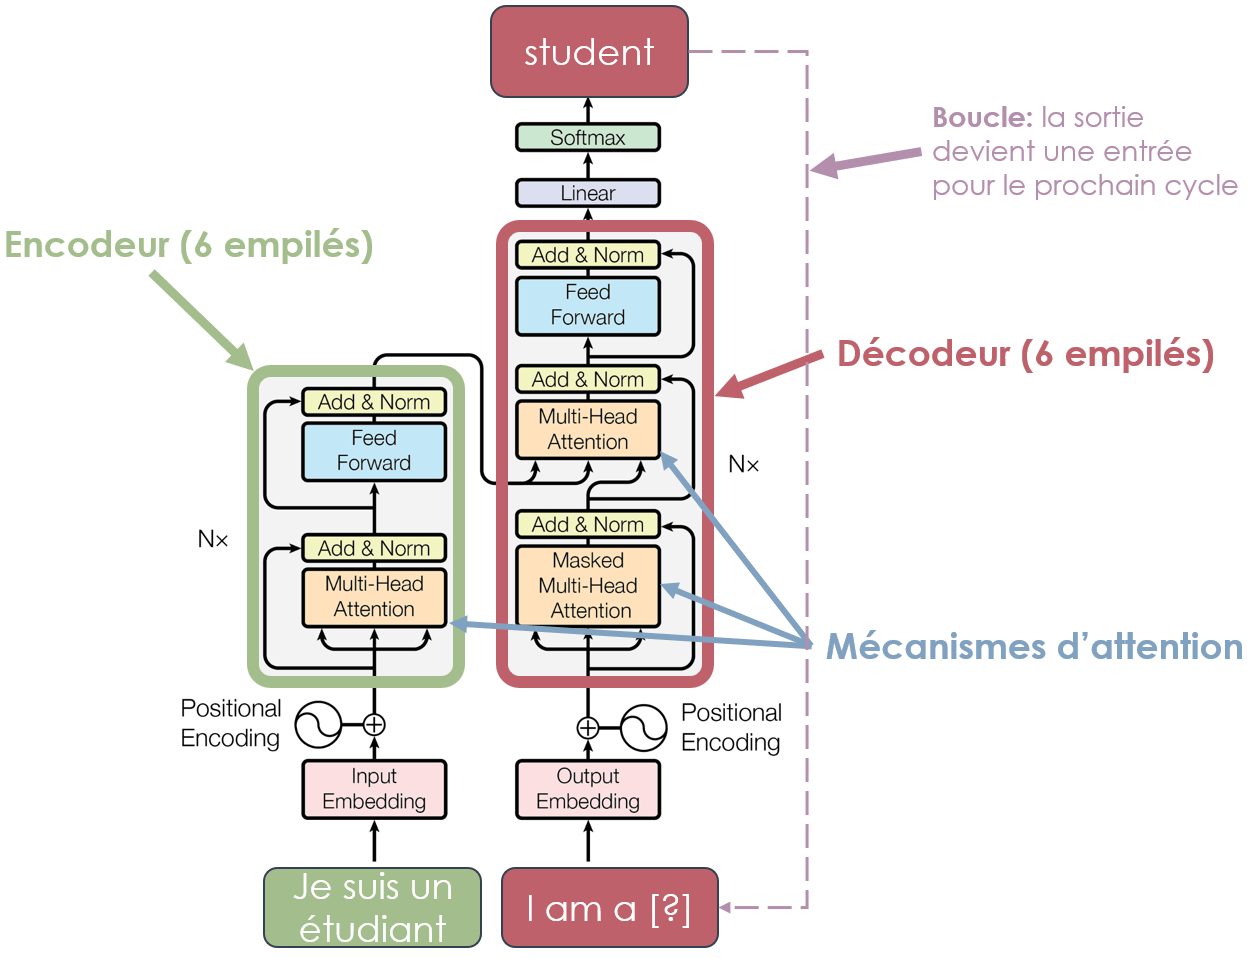
\includegraphics[width=1\textwidth]{figures/transformer.png}
 \caption[Schéma de l'architecture d'un réseau Transformer]{\textbf{Schéma de l'architecture d'un réseau transformer.} Les transformer sont composés de 6 encodeurs empilés (en vert), reliés à 6 décodeurs empilés (en rouge), chacun composé de mécanismes d'attention (en bleu). Les prédictions du modèle se font suivant une boucle (en violet) où à chaque étape, la prédiction actuelle est utilisée comme entrée pour la prédiction suivante.}
 \label{fig:transformer}
\end{figure}

Ici pour expliquer le fonctionnement des \textit{transformers}, nous avons utilisé l'exemple de la traduction de texte. Mais les \textit{transformers} peuvent être utilisable pour n'importe quelles données séquentielles, telles que les séquences génomiques et protéiques. Il est possible de considérer les séquences d'ADN et de protéine comme un simple enchainement de lettres, un nouveau langage à traduire. Nous allons voir deux exemples d'utilisation de \textit{transformers} pour l'analyse de séquences biologiques à travers Enformer et AlphaFold.

\subsection{Enformer: un \textit{transformer} pour l'expression des gènes}
Comme écrit précédemment, l'expression des gènes dans le génome est modulée par des interactions longue distance, grâce notamment aux \textit{enhancers}. Ainsi, si l’on veut construire des modèles prédictifs de l'expression des gènes, il faut avoir une architecture capable de considérer ces interactions longue distance, c'est précisément l'intérêt des \textit{transformers}. Dans les travaux intitulés "\textit{Effective gene expression prediction from sequence by integrating long-range interactions}" (\cite{avsec_effective_2021}) publié en 2021, une équipe de DeepMind a utilisé un modèle mixant convolutions et \textit{transformers} pour prédire l'expression des gènes (figure \ref{fig:enformer}. Là où le précédent modèle n'était capable de prendre que 20 000 paires de bases de contexte autour d'un gène pour effectuer sa prédiction, ce nouveau modèle nommé \textit{Enformer} est capable d'étendre le contexte jusqu'à 100 000 paires de bases en amont et en aval du gène. Grâce à l'examen des prédictions réalisées, ils ont réussi à mettre en évidence que le modèle a porté son attention sur la présence d'\textit{enhancers} localisés à 50 000 paires de bases du gène. Ce qui confirme l'intérêt de l'utilisation de \textit{transformers} dans le cadre de l'analyse de l'expression des gènes et de la prise en compte des \textit{enhancers}. Cependant, de récents travaux (\cite{karollus_current_2023}) ont montré que même pour le modèle \textit{Enformer}, la prise en compte des éléments distants reste un défi, car ils ont un poids moindre dans les prédictions du modèle par rapport aux éléments proches. \clearpage

\begin{figure}[H]
 \centering
 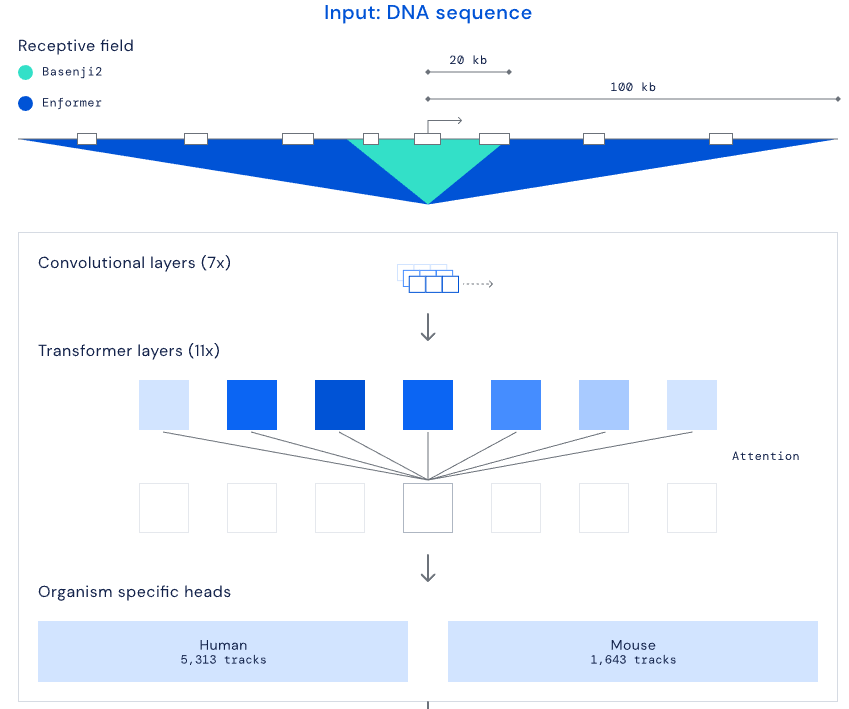
\includegraphics[width=0.8\textwidth]{figures/enformer.png}
 \caption[Schéma de l'architecture du modèle enformer]{\textbf{Schéma de l'architecture du modèle enformer.} Ce modèle basé sur les \textit{transformers} permet de prendre jusqu'à 100 000 paires de bases de contexte génomique pour évaluer l'expression d'un gène (\cite{avsec_effective_2021}).}
 \label{fig:enformer}
\end{figure}

\subsection{AlphaFold : un transformer pour la conformation 3D des protéines}
En 2020, le modèle AlphaFold 2 (\cite{jumper_highly_2021}) a remporté la CASP14 (\url{https://predictioncenter.org/casp14/}), compétition de référence dans le domaine de la prédiction de structure protéique. Leur modèle a obtenu un score global de 244 (somme de z-scores), contre 90,8 pour le second meilleur modèle (\cite{jumper_applying_2021}). Une des caractéristiques principales du modèle AlphaFold est l'usage d'une architecture similaire aux \textit{transformers} (figure \ref{fig:alphafold}). Ces blocs nommés "\textit{evoformers}" utilisent les mêmes mécanismes d'attention à l'œuvre dans la structure classique des \textit{transformers}. Comme dans le contexte génomique, les interactions 3D qui ont lieu dans les séquences protéiques ne sont pas que locales, ainsi il est nécessaire de pouvoir prendre en compte des interactions longue distance pour obtenir une prédiction de qualité, grâce à ces mécanismes d'attention. L'utilisation de cette architecture a permis le développement d'un outil qui révolutionne le domaine de la biologie structurale rendant possible l'accès à la structure 3D prédite de n'importe quelle protéine du vivant.

\begin{figure}[htbp]
 \centering
 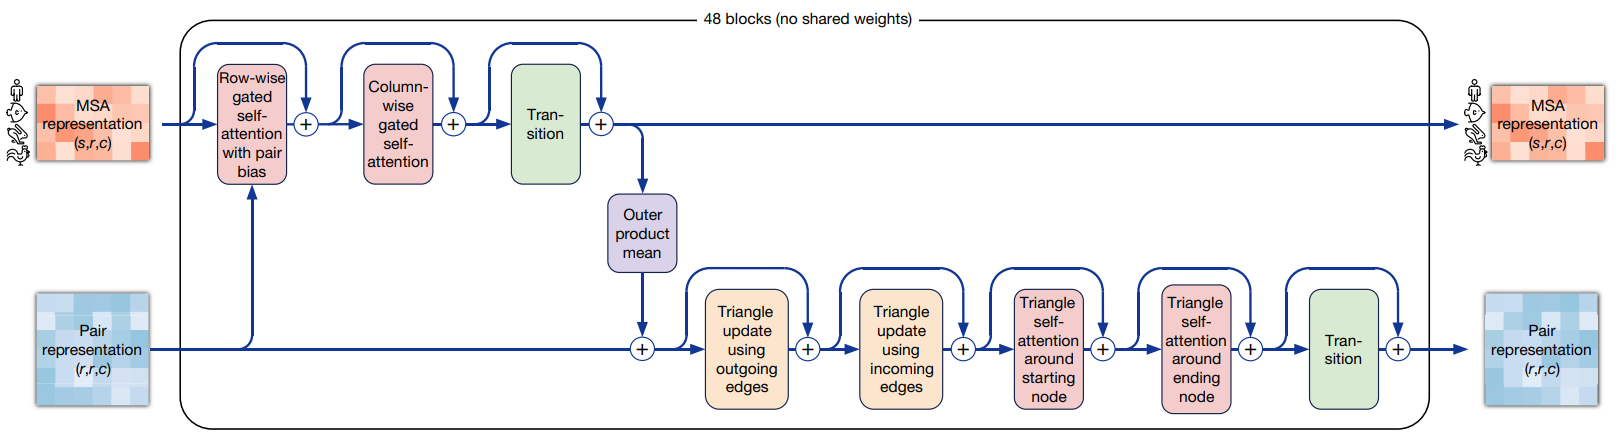
\includegraphics[width=1\textwidth]{figures/alphafold.png}
 \caption[Schéma de l'architecture du modèle AlphaFold]{\textbf{Schéma de l'architecture du modèle AlphaFold.} Ce modèle utilise les mécanismes d'attention des transformers pour prédire la conformation 3D de protéines à partir de leurs séquences et alignements.}
 \label{fig:alphafold}
\end{figure}

Bien que les \textit{transformers} présentent une grande avancée dans le domaine des \gls{dnn} avec la prise en compte des interactions longue distance, ils présentent un certain nombre de limites qui doivent être considérées avant leur utilisation. Tout d'abord en terme de cout de calcul, les \textit{transformers} par leurs mécanismes d'attention (processus quadratique) sont très couteux en mémoire et en ressources pour le traitement de longues séquences. Par exemple, Alphafold ne prédit que les protéines d'une taille inférieure à 150 acides aminés en raison de la complexité des calculs nécessaires, ce qui exclut un certain nombre de protéines humaines, dont la titine, une protéine essentielle à la structure des muscles. Ensuite, les \textit{transformers} ont besoin d'une quantité de données plus importantes pour leur entrainement que des architectures moins complexes, ce qui peut être un problème dans le domaine biomédical (\cite{willemink_toward_2022}). Enfin, alors que pour les \gls{cnn} il existe des méthodes d'explicabilité \textit{ad-hoc}, les \textit{transformers} étant plus complexes et récents, les techniques d'explicabilité à disposition sont moindre, mais c'est un domaine de recherche actif (\cite{kim_can_2022, saha_explainability_2022}). 

Ainsi l'utilisation des \textit{transformers} est à réserver pour les tâches qu'on ne peut pas résoudre par des architectures plus simples. Une de ces tâches est la compréhension du langage naturel, donc l'architecture \textit{transformer} a permis de révolutionner le traitement grâce aux \gls{llms} que nous présentons dans la prochaine section.

\subsection{Traitement de langage naturel pré modèle linguistique de grande taille}
Le \gls{nlp} est une branche de l'\gls{ia} qui s'intéresse à la compréhension du langage humain de manière automatique. Le \gls{nlp} est très utile par exemple pour exploiter et extraire de l'information de comptes rendus médicaux en texte libre. Les méthodes traditionnelles de \gls{nlp} reposent sur le concept d'ontologies, présentées dans le premier chapitre (\ref{onto_ref}). Cette méthode se base sur une recherche de correspondance exacte des mots d'un texte par rapport à l'ontologie. Cette approche a été implémentée dans divers outils, comme \textit{EMERSE} (\cite{hanauer_supporting_2015}), pour extraire de l'information des dossiers de santé électroniques de patients. Cependant, elle présente des limites importantes: le besoin d'établir une ontologie exhaustive avec des synonymes, dans la même langue que le texte et que le texte soit exact (sans erreurs d'orthographe ni d'acronymes).

Des méthodes plus flexibles basées sur \gls{ia} par réseaux de neurones (hors transformers) ont été développées. Ces méthodes reposent sur l'entrainement de réseau de neurones pour la détection et l'extraction d'informations de textes (symptômes, gènes, nom de maladies...). Cette approche a permis le développement, par exemple, de \textit{DeepPhe} (\cite{savova_deepphe_2017}), un outil d'extraction de phénotypes à partir de comptes rendus cliniques ou encore les modèles intégrés dans \textit{SciSpacy} (\cite{neumann_scispacy_2019}) capables de détecter et de classer les termes biomédicaux relatifs aux cellules, acides aminés, noms de gènes, noms de maladies, protéines, organismes, tissus, organes et autres. Ces méthodes sont plus robustes que celles basées sur les ontologies, car elles sont résistantes aux erreurs dans le texte et reposent sur une compréhension sémantique des termes et non sur une correspondance exacte de mots. Mais elles présentent tout de même encore des limites. En effet, ces méthodes sont spécifiques à une seule tâche de reconnaissance et à une langue, elles ne peuvent pas suivre des instructions. S’il n'existe pas de modèles de reconnaissance des termes histologiques ou de modèles entrainés sur des comptes rendus français, il est alors nécessaire de ré-entrainer un modèle à partir d'un nouveau jeu de données. 

Les modèles de types \textit{transformers} et plus spécifiquement les \gls{llms} révolutionnent le domaine du \gls{nlp} en permettant de dépasser les limites des méthodes précédentes. Ces grands modèles dits "Modèles de fondation" (\textit{foundation models}) sont présentés plus en détail dans la section suivante.

\subsection{La ruée vers l'or des modèles linguistiques de grande taille}\label{chap2_llms}
Les années 2022-2023 représentent des années clés dans l’histoire de l'analyse et la compréhension de texte (\gls{nlp}) avec le développement et la mise à disposition de plusieurs modèles de fondation généraux performants et accessibles tel que \textit{GPT-3.5-turbo} (souvent nommé à tort \textit{ChatGPT)} ou \textit{LLaMA} (\cite{touvron_llama_2023}). Ces \gls{llms} représentent une véritable révolution dans le traitement des données textuelles non structurées, car ils sont capables de suivre des instructions précises et extrêmement variées, dans de multiples langues et de manière robuste face aux erreurs dans le texte. Dans un long papier de 155 pages nommé "\textit{Sparks of Artificial General Intelligence: Early experiments with GPT-4}" publié en avril 2023 par une partie de l'équipe ayant travaillé sur le modèle GPT-4 d'OpenAI (\cite{bubeck_sparks_2023}), les auteurs dressent un portrait des capacités des \gls{llms} et de leur possible impact sociétal.

Pour ne citer que quelques exemples des capacités des \gls{llms}, ces modèles sont capables de résumer des articles scientifiques en une série de points clés, de générer du code informatique et d'en corriger les erreurs, d'extraire des informations spécifiques d'un texte, de répondre à des questions de logique, d'expliquer des blagues, d'écrire des histoires créatives, d'analyser des images et d'interagir avec le monde extérieur par des requêtes internet. Ces modèles ont donc des capacités extrêmement vastes avec des performances proches de l'Homme. Les modèles \gls{llms} sont très divers et en constante évolution. La figure \ref{fig:llm-tree} (\cite{yang_harnessing_2023}) retrace les principaux modèles développés entre 2018 et 2023 où l'on observe une nette évolution entre 2022 et 2023 avec une multitude de modèles ouverts ou fermés développés. 

\begin{figure}[htbp]
 \centering
 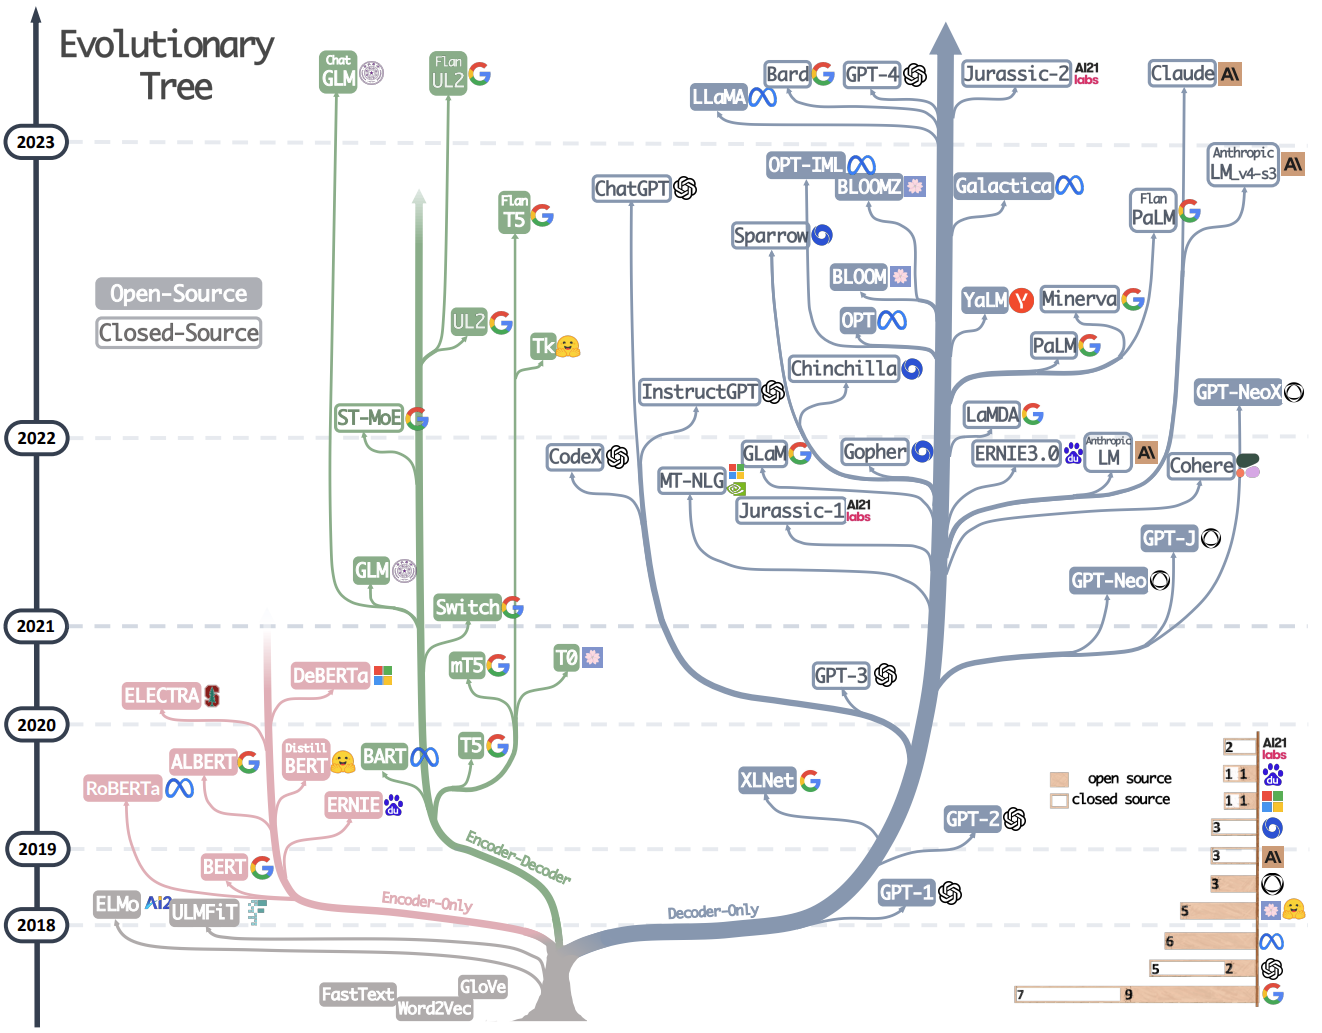
\includegraphics[width=1\textwidth]{figures/llm_tree.png}
 \caption[Arbre du développement LLMs de 2018 à 2023 (\cite{yang_harnessing_2023})]{\textbf{Arbre du développement LLMs de 2018 à 2023}. On observe à partir de 2022 une forte croissance du nombre de modèles développés pour l'analyse de texte basés sur les architectures de \textit{transformers}. (\cite{yang_harnessing_2023})}
 \label{fig:llm-tree}
\end{figure}

Cette évolution et accélération de la recherche que j'ai choisi de qualifier de "ruée vers l'or" traduit un net engouement pour ces modèles et des tâches qui peuvent être accomplies. Cette émulation de la recherche en \gls{ia} autour des \gls{llms} a mené au développement de modèles de toutes tailles et de tous types ainsi qu'au développement d'infrastructures et de techniques pour l'hébergement, l'optimisation et l'utilisation de ces nouveaux modèles. Le développement de tels modèles a été rendu possible par l'utilisation de deux innovations en plus des \textit{transformers}: l'\gls{ssl} et l'\gls{rlhf} que nous allons brièvement présenter ci-dessous.

\subsubsection{Apprentissage auto-supervisé}
En mars 2021, Yann Lecun a écrit un billet de blog qualifiant l'apprentissage auto-supervisé comme la matière noire de l'intelligence \textit{(Self-supervised learning: The dark matter of intelligence}, \cite{lecun_self-supervised_2021}). Dans ce billet, il explique que l'apprentissage auto-supervisé est l'une des voies les plus prometteuses pour construire des connaissances de fond dans les modèles \gls{ia}.

L'idée dernière le \gls{ssl} part d'un constat: l'ensemble des modèles d'\gls{ia} nécessitent un jeu de données bien annotées pour leur entrainement. Or, il est facile d'acquérir un grand nombre de données non annotées, le goulot d'étranglement se situe dans l'annotation et la labellisation des jeux de données. Par exemple, il est facile d'acquérir un grand nombre de pages internet et d'en extraire le texte. Comment utiliser ces données non annotées pour entrainer un modèle de langage ? Est-il possible de définir une méthode d'apprentissage à partir des données non annotées ? C'est précisément l'intérêt du \gls{ssl}.

Le fonctionnement du \gls{ssl} est relativement simple. Dans une phase de pré-entrainement, le modèle va apprendre à recréer les données qui lui sont fournies. Par exemple, si l'on veut créer un modèle de langage, on peut lors de ce pré-entrainement lui fournir une phrase telle que: \\
"Les modèles \gls{ia} sont des systèmes complexes capables de réaliser des prédictions". \\
Pour le pré-entrainement du modèle par \gls{ssl} on va cacher certains mots de la phrase et entrainer le modèle à prédire le mot attendu. Ainsi on obtient la phrase: \\
"Les modèles \gls{ia} sont des systèmes [?] capables de réaliser des [?]". \\
Et pour chaque point d'interrogation, le modèle va être entrainé à prédire les mots "complexes" et "prédictions" avec une grande probabilité. Par cette méthode, il est possible d'utiliser des données non annotées pour réaliser un pré-entrainement qui permet au modèle une meilleure compréhension de la structure d'un texte et de la relation entre les mots. Après ce pré-entrainement, l'entrainement classique du modèle peut avoir lieu, avec un nombre de données annotées plus limité que sans le pré-entrainement par \gls{ssl}.

Le concept de \gls{ssl} n'est pas limité au texte, le principe est similaire avec des images. Par exemple, il est possible de diviser une image en 16 zones carrées, de masquer une de ces zones et d'entrainer le modèle à régénérer la zone en guise de pré-entrainement. Pour cela, le jeu de données ImageNet (\cite{deng_imagenet_2009}) est communément utilisé. Ce jeu de données est composé de plus de 14~millions d'images réparties sur 1000 classes différentes et variées (animaux, objets, fruits, bâtiments). Il est typiquement utilisé comme méthode d'évaluation des performances des nouvelles architectures de réseaux de neurones. Il a été montré qu'un pré-entrainement sur ImageNet par \gls{ssl} permet d'obtenir de meilleures performances de classification avec une quantité de données moindre (\cite{goyal_self-supervised_2021})

\subsubsection{Apprentissage par renforcement avec retour humain}
L'apprentissage par renforcement avec retour humain est une méthode qui a permis l'amélioration des performances des \gls{llms} (\cite{ziegler_fine-tuning_2020, stiennon_learning_2020}). Cette méthode permet non seulement de réduire les biais dans le modèle grâce à une intervention humaine (biais raciaux, de genre, religieux, \cite{ganguli_red_2022}), mais aussi de créer un modèle capable de suivre des instructions (\cite{ouyang_training_2022}).

Après le pré-entrainement par \gls{ssl} et l'entrainement classique du modèle avec des données annotées, les sorties du modèle vont être affinés par apprentissage par renforcement. Plusieurs exemples de générations pour une instruction vont être présentés à un humain qui va devoir classer les réponses dans un ordre de préférence. Le modèle va ainsi obtenir une pénalité ou une récompense pour chaque réponse, ce qui permet d'affiner ses futures réponses. Ainsi le retour humain est intégré à l'entrainement du modèle par ce mécanisme d'apprentissage par renforcement pour rentre le modèle moins biaisé et qualitatif.

\subsection{Les modèles génératifs et modèles d'\textit{embedding}}
Les \gls{llms} se déclinent sous deux formes principales avec des utilisations différentes: les modèles génératifs et les modèles d'\textit{embedding}. La figure \ref{fig:llm-type} présente les deux types de modèles.

\begin{figure}[htbp]
 \centering
 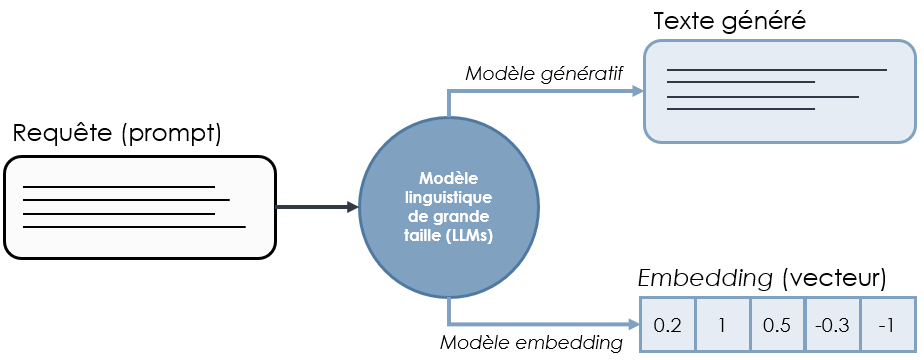
\includegraphics[width=1\textwidth]{figures/two_llm.png}
 \caption[Schéma des deux types de LLMs principaux]{\textbf{Schéma des deux types de LLMs principaux}. D'un côté, il y a les modèles génératifs qui sont des modèles de complétions, produisant du texte à partir de texte. De l'autre, les modèles d'\textit{embedding} transforment le texte d'entrée en vecteur numérique de grande taille représentant le sens sémantique du texte d'entrée.}
 \label{fig:llm-type}
\end{figure}

Les modèles de type \textit{embedding} consistent à transformer un texte d'entrée en vecteur numérique de grande taille. L'idée derrière cette transformation est que deux phrases ayant un sens similaire (sens sémantique) ont une représentation numérique similaire. Transformer le texte en vecteur numérique permet de réaliser des opérations, telles que la recherche de similarité entre deux phrases, mais aussi le \textit{clustering}, la visualisation graphique ou encore l'entrainement de modèles de classification. Le concept d'\textit{embedding} est donc un réel couteau suisse pour l'analyse et la recherche de similarité entre des textes et il est en général multilingue: deux phrases identiques, mais dans des langues différentes vont avoir une représentation numérique similaire. La figure \ref{fig:sentence_embed} (\cite{luis_serrano_what_2023}) présente une visualisation de l'\textit{embedding} de 9 phrases en deux dimensions. On observe sur cette figure que les phrases traitant d'un sujet similaire sont regroupées en sous-groupe dans l'espace. On observe un groupe qui concerne les chiens, un groupe concernant le football et un groupe concernant une question de type "comment vas-tu". Cet exemple est simplifié à des fins de représentation, car les phrases ne sont encodées qu'en deux dimensions. En réalité pour capturer des nuances complexes dans les phrases, les modèles d'\textit{embedding} encodent les phrases en plusieurs centaines voire en milliers de dimensions.

\begin{figure}[htbp]
 \centering
 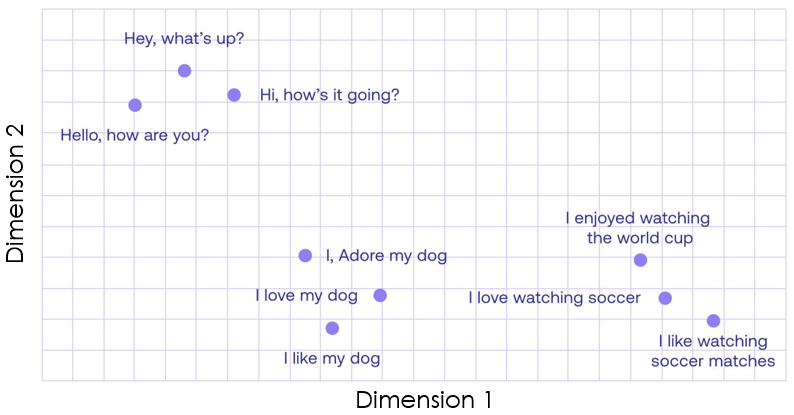
\includegraphics[width=0.66\textwidth]{figures/sentence_embed.png}
 \caption[Visualisation d'embedding de 9 phrases en 2 dimensions]{\textbf{Visualisation d'embedding de 9 phrases en 2 dimensions}. Dans cette représentation en deux dimensions, on observe que les phrases qui concernent des sujets similaires se regroupent dans l' espace en clusters, indiquant que leurs représentations numériques (par \textit{embedding}) sont similaires. (\cite{luis_serrano_what_2023})}
 \label{fig:sentence_embed}
\end{figure}

Les modèles génératifs sont des modèles de complétion. À partir d'un texte en entrée, ils génèrent un texte de sortie. Ces modèles sont utiles pour des tâches créatives comme la génération d'histoires ou de code, mais aussi pour suivre des instructions précises telle l'extraction d'informations d'un texte comme la récapitulation d'un article scientifique. Le texte en entrée contenant les instructions pour le modèle est nommé \textit{prompt} (figure \ref{fig:llm-prompt}). Le défi dans l'utilisation des modèles génératifs réside dans la création d'un \textit{prompt} adapté aux résultats que l'on souhaite obtenir. Le processus de création et d'affinage d'un \textit{prompt} pour une tâche se nomme "\textit{prompt engineering}". Classiquement, un \textit{prompt} possède une structure de base en quatre éléments: (i) la description précise de la tâche (ii) un exemple de réalisation de la tâche et de résultat souhaité(iii) le texte que l'on souhaite analyser (iv) un indicateur de sortie indiquant au modèle qu'on attend une réponse. L'avantage des modèles génératifs réside dans le fait qu'aucun apprentissage supplémentaire n'est nécessaire, le point central étant l'établissement d'un \textit{prompt} optimal.

\begin{figure}[htbp]
 \centering
 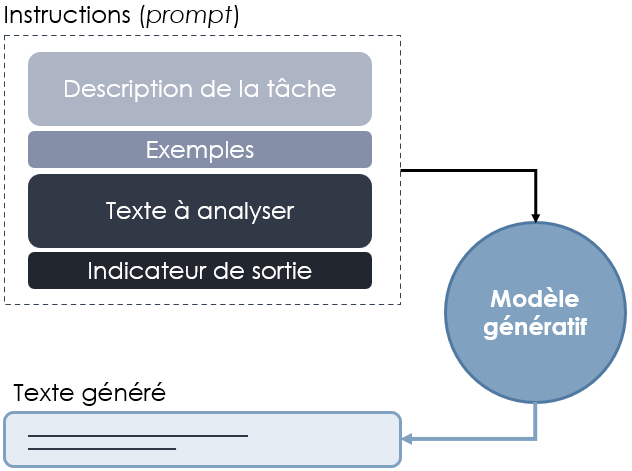
\includegraphics[width=0.66\textwidth]{figures/promt_llm.png}
 \caption[Schéma du concept de \textit{prompt} pour les LLMs génératifs]{\textbf{Schéma du concept de \textit{prompt} pour les LLMs génératifs}. Un \textit{prompt} typique est constitué de quatre parties: (i) une description de la tâche, (ii) un exemple de réalisation de la tâche, (iii) le texte à analyser en entrée, et (iv) un indicateur de sortie.}
 \label{fig:llm-prompt}
\end{figure}

\subsection{Taille des modèles et défis d'utilisation}
Les \gls{llms} sont très versatiles et peuvent accomplir de nombreuses tâches, mais ils restent une technologie très récente en constante évolution et encore peu optimisée. Bien que les modèles d'\textit{embedding} sont très facilement utilisables sur presque n'importe quel matériel informatique, les modèles génératifs quant à eux sont en général d'une taille extrême rendant leur hébergement très compliqué. Comme déjà abordé dans la section "Nombre de paramètres et ressources informatiques" ci-dessus, les \gls{llms} peuvent avoir une taille allant de 10 à plusieurs centaines de milliards de paramètres, rendant difficile leur adoption et leur utilisation.

Pour rendre ces modèles accessibles, plusieurs stratégies existent. La première est la mutualisation de l'hébergement, où une entité (une entreprise, un laboratoire), va héberger sur du matériel informatique spécialisé un \gls{llms} qui va être disponible \textit{via} des requêtes internet (\gls{api}). Cette solution pose des problèmes de confidentialité des données. 

La deuxième stratégie est d'optimiser les modèles de grande taille. Une première méthode d'optimisation utilisée est nommée la quantisation (\cite{dettmers_case_2023, dettmers_llmint8_2022}) qui consiste à réduire la complexité informatique des poids des modèles. Les poids des modèles sont représentés par des nombres décimaux sur 16 bits informatiques (65 536 valeurs possibles). Il est possible de réduire cette complexité en représentant les poids du modèle sur seulement 4 bits (16 valeurs possibles) avec une perte minimale en précision, ce qui permet de réduire d'un facteur 4 la taille du modèle et les couts d'hébergement.

La troisième stratégie est d'entrainer des modèles de plus petite taille à partir des sorties de modèles de grande taille, afin de les "imiter". Ainsi, il a été possible d'entrainer de petits modèles avec seulement 7~milliards de paramètres (contre 175 milliards pour GPT-3) à partir de 52 000 exemples de générations de textes de grands modèles (\cite{peng_instruction_2023}). Cependant, de récents travaux (\cite{gudibande_false_2023}) ont montré que cette approche bien qu'efficace en apparence, n'est pas capable d'imiter l'ensemble des capacités des modèles de très grande taille.

Pour conclure ce chapitre, il est clair que les méthodes présentées permettent d’explorer de façon rétrospective et multimodale, de nombreuses données biomédicales acquises sur des patients, qu'elles soient textuelles, d'imagerie ou de séquences. Ces méthodes, bien que complexes à mettre en place et à utiliser, permettent de combler les limites du \gls{ml} présenté dans le chapitre précédent et ouvrent la porte à l'exploitation de données sans nécessiter un travail d'annotation et de structuration intensif. La stratégie de couplage de réseaux de neurones comme extracteurs d'informations de données non structurées avec des algorithmes de \gls{ml} transparents et explicables apparait prometteuse pour l'exploitation des données biomédicales non structurées. Dans le prochain chapitre, nous présenterons un cas d'application de ces nouvelles méthodes à travers les myopathies congénitales, une famille de maladies génétiques rares. Nous présenterons leur diagnostic et les données associées à celui-ci.